
\chapter{Neutrino Physics}


Since its original inception in the 1930s, neutrino physics has developed into a robust field of high energy physics.  The neutrino was theorized in the 1930s by Wolfgang Pauli, rigorously incorporated into the theory of beta decay by Enrico Fermi \cite{Fermi}, and first detected in 1956 by Clyde Cowan and Frederick Reines \cite{cowanReines}.

Originally, the neutrino was postulated to preserve conservation of momentum in the theory of beta decay, where a nucleon such as a neutron is converted to a proton by emitting an electron and a neutrino:
\begin{equation}
\label{beta_decay}
n \rightarrow p^+ + e^- + \nuebar
\end{equation}

The reaction above is actually an example of a weak interaction happening at the quark level, where one of the neutron's down quarks converts to an up quark through the emission of a $W^-$.  Unfortunately, the neutrino is a very weakly interacting particle, so the direct observation of both the electron and the neutrino from a $\beta$ decay reaction was, and still is, impossible.  

For the detection of the neutrino, Cowan and Reines used a very similar reaction to beta decay, but instead of producing a neutrino this reaction absorbs a neutrino and emits a neutron and a positron:
\begin{equation}
\label{inverse_beta_decay}
p^+  + \nuebar \rightarrow e^- + n 
\end{equation}

Unlike neutrinos, neutrons and positrons are relatively easy to observe, so Cowan and Reines simply exposed a large sample of protons to a very large blast of neutrinos.  Practically, this meant building a detector near a high intensity source of neutrinos, which they did: they exposed large tanks of water to the neutrino flux of a nuclear reactor at the Savannah River plant, in Georgia.  The neutrinos coming to their detector (actually, {\em anti}-neutrinos) interacted with the protons and produced a neutron and a positron.  The positron was observed after it interacted by annihilating with an electron in the water tank, producing a pair of gamma particles.  The neutron was detected by it's capture on Cadmium, which was doped in the tank.  The neutron capture also produces a gamma, but it is delayed from the positron's gamma pair.  Cowan and Reines ultimately observed about three neutrinos per hour in their detector.  Conclusively, when the reactor was shut off, they no longer observed neutrinos. 

Since the first discovery of the neutrino, neutrinos and their interactions have played a central role in the development of the standard model of particle physics.  Pauli originally proposed only one neutrino, but not long after his prediction (and before the experimental evidence that confirmed it) other types of neutrinos were postulated.   Since then, 2 other types of neutrinos have been discovered, namely the muon and tau neutrinos \cite{muon_neutrino},\cite{tau_neutrino}. 

Conventionally, neutrinos are symbolized as $\nu_e, \nu_\mu,$ and $\nu_\tau$ corresponding to the 3 flavors of charged leptons.  The charged current interactions of these neutrinos, by exchanging a $W^\pm$ boson, produces an outgoing charged lepton of the same flavor as the incoming neutrino: \nue produces electrons, \nuebar produces anti-electrons, \numu produces muons, etc, such as in Equations~\ref{beta_decay} and \ref{inverse_beta_decay}.  However, neutrinos can also interact via neutral currents, where the outgoing lepton is {\em not} charged.  Instead, the neutrino exchanges a neutral $Z^0$ boson with the target material.  The first observed neutral current interaction is shown in Figure~\ref{fig:gargamelle_nc} \cite{gargamelle_nc}.

\begin{figure}[htbp]
  \centering
  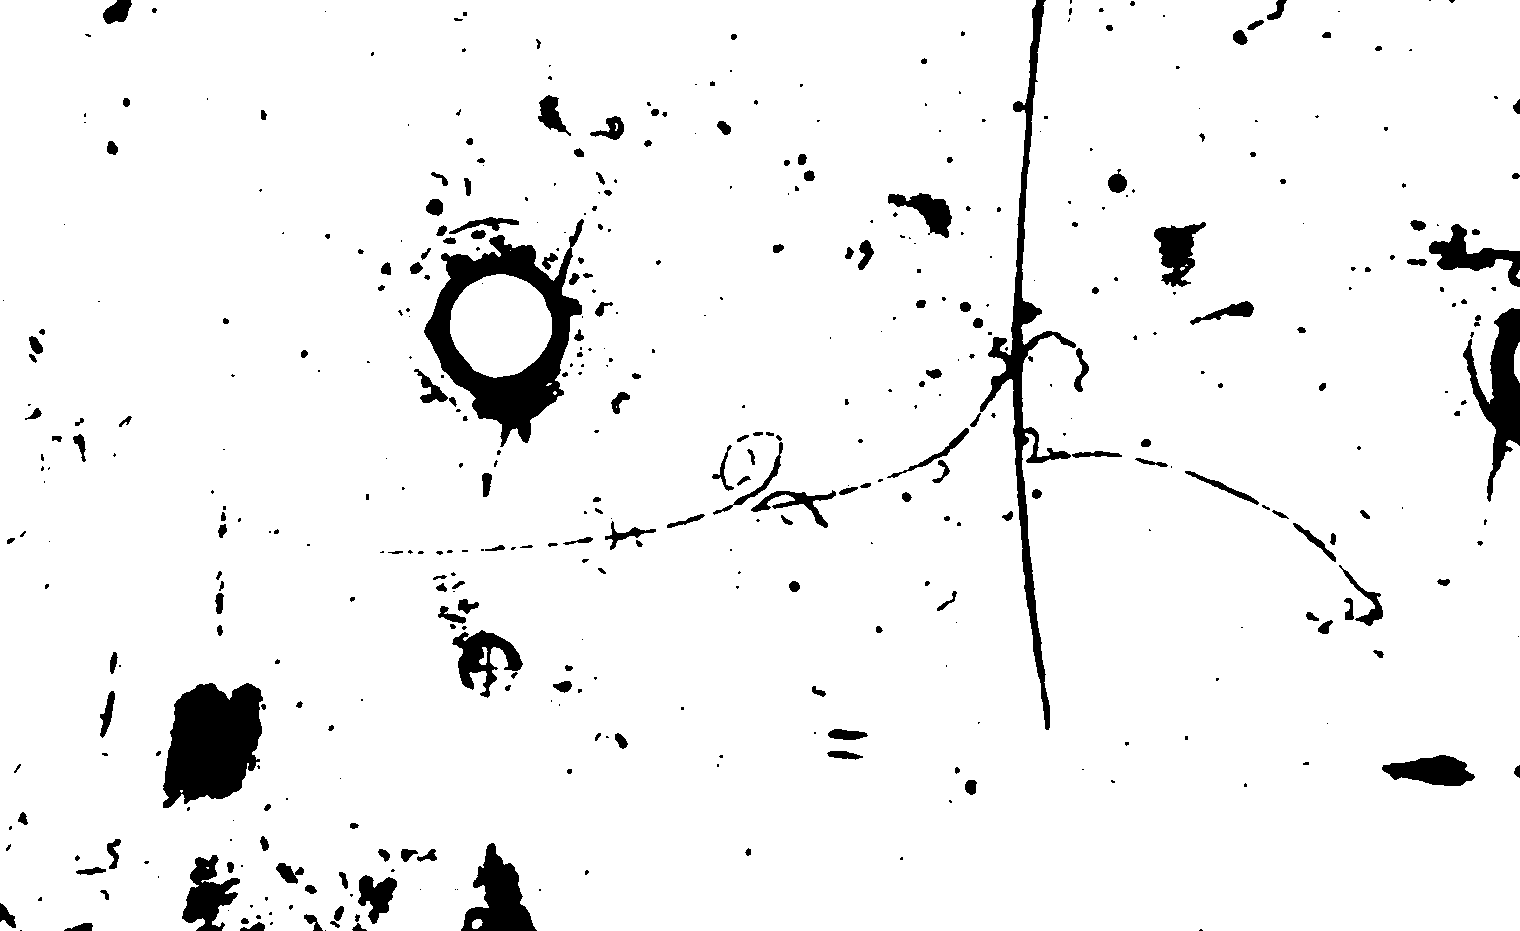
\includegraphics[width=0.95\textwidth]{intro_figures/gargamelle_nc.png}
  \caption[First Observed Neutral Current Neutrino Interaction]{The first observed neutral current neutrino interaction, seen by Gargamelle in 1973.}
  \label{fig:gargamelle_nc}
\end{figure}


Neutrino physics was dramatically altered with the discovery of neutrino oscillations, described below, which opens the door to measurements of CP Violation and possible sterile states of neutrinos.  Since the 1960s until the early 2000s, the field of neutrino physics had an unresolved anomaly known as the Solar Neutrino Problem.  Models of the interactions in the interior of the sun made a definite prediction for the number of electron-flavor neutrinos arriving at Earth \cite{solar_neutrinos}, based on well grounded theories of stellar fuel burning.  On the other hand, experiments sensitive to neutrinos observed a significant deficit as compared to predictions \cite{davis}.  It wasn't until the GALLEX/SAGE \cite{gallex} \cite{sage} experiments, along with the Super-Kamiokande experiment \cite{superK} and the Sudbury Neutrino Observatory \cite{SNO}, that a solution to the Solar Neutrino Anomaly was found through the mechanism of oscillations: the sun did in fact produce the predicted rate of electron neutrinos, but experiments that were only sensitive to electron neutrinos were unable to detect the muon and tau neutrinos that were produced through the oscillation mechanism.  

The conclusive evidence for neutrino oscillations also implies that neutrinos are not, as was initially believed, massless particles.  However, neutrinos are known to be incredibly light weight, and cosmological constraints imply neutrinos have a mass of less than  XX \cite{cosmological_neutrinos}.  The exact mass of each type of neutrino is unknown still, though experiments are setting lower and lower bounds to directly constrain it \cite{katrin}.

One of the most exciting questions that may be addressed by studying neutrinos is CP violation.  Some theories predict that the current matter/anti-matter imbalance in the observable universe can be explained by CP violation by leptons, such as neutrinos. \cite{CP_theories}  This parameter is directly probable with neutrinos by measuring the difference in neutrino oscillations between neutrinos and anti-neutrinos, as described below.  In particular, the neutrino matter effect \cite{matter_effect} leads to a large observable effect of CP violation in electron neutrinos.

Another intriguing avenue of discovery in neutrino physics is the resolution of short baseline anomalies, which may hint towards the existence of sterile neutrinos.  Experiments have been proposed to probe these anomalies \cite{SBN, prospect}, and other existing experiments have found ways to investigate short baseline anomalies already \cite{icecube, nova_steriles, minos_steriles, daya_bay_steriles}.

Both for the case of CP violation and the resolution of short baseline anomalies, the detection and measurement of electron neutrinos crucial.  The most promising proposal to measure CP violation, DUNE \cite{DUNE}, will look for the appearance of electron neutrinos in a primarily muon neutrino beam.  The Fermilab Short Baseline Neutrino Program (SBN Program) \cite{SBN} will similarly be searching for electron neutrinos in a primarily muon neutrino neutrino beam.  The first stage of the SBN Program, \uboone, is already running in Fermilab's Booster Neutrino Beam searching for low energy electron neutrinos.

Both DUNE and the SBN Program rely on high granularity detectors for their neutrino searches, the liquid argon time projection chamber (LArTPC, see Chapter~\ref{chp:lartpc}).  However, at the time of the publication of this thesis, only one \lartpc in the world has ever observed electron neutrinos.  The ICARUS experiment includes an observation of two electron neutrinos at approximately 20 GeV \cite{ICARUS_steriles}.  On the other hand, the energy of interest to both DUNE and SBN is significantly lower, in the range of 1 GeV.  Therefore, the work presented in this thesis is the first observation of low energy electron neutrinos in a liquid argon time projection chamber.   



\section{Neutrino Sources}

Neutrinos, despite their weak interaction cross section and difficulty to observe, are actually incredibly common on Earth - more than a trillion neutrinos pass through an average sized human hand every second.  By far the most powerful nearby source of neutrinos is from the Sun, produced predominantly in proton-proton fusion.  But, more powerful (and more exotic) sources of neutrinos are known to exist, such as supernova \cite{supernova_1987a}.  Terrestrially, neutrinos are produced in the geothermal reactions of the Earth's core, and there is large flux of ``atmospheric'' neutrinos produced by the interactions of cosmic particles in the upper atmosphere.  As radioactive elements decay through weak interactions, radioactive material emits neutrinos as well - in fact this can be a quite useful source for calibration of neutrino experiments.

There are also artificial sources of neutrinos, most commonly nuclear reactors.  Though they are less powerful than the Sun, neutrino experiments can get significantly closer to a nuclear reactor than to the Sun, and the local neutrino flux can be quite high.  The most sophisticated artificial source of neutrinos comes from the neutrinos beams produced at accelerator complexes such as Fermilab, CERN, and J-PARC.  Artificial neutrino beams can provide a high intensity source of neutrinos over a large range of energies, and offer many other benefits as well.  

A detailed understanding of the source of neutrinos is vital to the success of every neutrino experiment, and Chapter~\ref{chp:beams} explores neutrino beams in more detail.

\subsection{Solar Neutrinos}

\subsection{Atmospheric Neutrinos}

\subsection{Supernova Neutrinos}

\subsection{Radioactive Sources}

\subsection{Reactor Neutrinos}

\subsection{Neutrino Beams}

\section{Neutrino Oscillations}

Neutrino oscillations are the foundation and the starting point for modern neutrino experiments exploring CP violation and short baseline anomalies, and can be used to probe the mass hierarchy of the neutrinos.  As such, they are fundamentally important to neutrino experiments, so a description of the theory of neutrino oscillations and the experimental evidence is presented here.

\subsection{Neutrino Oscillations - Theory}


Neutrinos, when produced through electro-weak interactions, are produced in flavor eigenstates.  To date, there are known to be three flavors of neutrinos: \nue, \numu, and \nutau.  Each of these neutrinos, as suggested by their name, corresponds to a charged lepton.  The conservation of lepton flavor, in electro-weak interactions, dictates that the number of leptons of a particular flavor is conserved during an interaction.  As an example, the decay of a muon to an electron would violate lepton flavor conservation if not for the presence of neutrinos:

\begin{equation}
\mu^- \rightarrow e^- + \bar{\nu}_e + \nu_\mu
\end{equation}

Lepton flavor violation is not, however, a law of nature.  The most striking evidence for the violation of lepton flavor conservation is neutrino oscillations, though there are hints and proposals that lepton flavor could be violated by charged leptons as well \cite{mu2e}.  For neutrino oscillations, the violation of lepton flavor is a direct result of the fact that neutrinos in the lepton eigenstates are a superposition of the mass eigenstates of neutrinos:

\begin{equation}
\nu_e = \alpha \nu_1 + \beta \nu_2 + \gamma \nu_3
\end{equation}

where the numerical neutrino states represent the neutrinos with a well defined mass.  It should be noted, from a historical perspective, that in fact neutrinos were originally considered to be zero-mass in the Standard Model.  The discovery of neutrino oscillations instead provided definitive evidence that neutrinos {\bf do} have mass.  From a modern perspective, however, the evidence for neutrino masses is overwhelming.  The interesting phenomenon, then, arise from the fact that neutrinos produce in lepton flavor states do not stay stably in those states.  

The most common way to mathematically describe neutrino oscillations is through the Pontecorvo-Maki-Nakagawa-Sakata matrix, or PMNS matrix:

\begin{equation}
  \left(
  \begin{array}{c}
    \nu_e \\
    \nu_\mu \\
    \nu_\tau \\
  \end{array}
  \right)
  =
  \left(
  \begin{array}{ccc}
    U_{e1} & U_{e2} & U_{e3}  \\
    U_{\mu1} & U_{\mu2} & U_{\mu3}  \\
    U_{\tau1} & U_{\tau2} & U_{\tau3}  \\
  \end{array} 
  \right)
  \left(
  \begin{array}{c}
    \nu_1 \\
    \nu_2 \\
    \nu_3 \\
  \end{array}
  \right)
\end{equation}

In this matrix, under the standard assumptions of neutrino oscillations, the rows and columns are normalize such that the matrix is  unitary: $\sum_{i=1}^3 | U_{\alpha i} | ^2 = 1$, and similarly for the columns.  It's very common for the PMNS matrix to be parameterize in terms of mixing angles: 

\begin{align*}
  \left(
  \begin{array}{ccc}
    U_{e1} & U_{e2} & U_{e3}  \\
    U_{\mu1} & U_{\mu2} & U_{\mu3}  \\
    U_{\tau1} & U_{\tau2} & U_{\tau3}  \\
  \end{array} 
  \right)
  = 
  \left(
  \begin{array}{ccc}
    1 & 0 & 0  \\
    0 & \text{cos}\theta_{23} & \text{sin}\theta_{23}  \\
    0 & -\text{sin}\theta_{23} & \text{cos}\theta_{23}  \\
  \end{array} 
  \right)
  &\times \\
  \left(
  \begin{array}{ccc}
     \text{cos}\theta_{13} & 0 & \text{sin}\theta_{13} e^{ - i \delta_{CP}}  \\
     0 & 1 & 0  \\
     -\text{sin}\theta_{13} e^{i \delta_{CP}} & 0 & \text{cos}\theta_{13}  \\
  \end{array} 
  \right)
  &\times \\
  \left(
  \begin{array}{ccc}
    \text{cos}\theta_{12} & \text{sin}\theta_{23} & 0  \\
    - \text{sin}\theta_{23} & \text{cos}\theta_{12} & 0 \\
    0 & 0 & 1  \\
  \end{array} 
  \right)
\end{align*}

The value of this expansion is that the individual mixing angles are observable with different experimental setups.  The additional phase, $\delta_{CP}$, is needed if neutrinos violate Charge-Parity symmetry.  Some theories suggest that neutrino violation of CP symmetry is responsible for the matter/anti-matter asymmetry in the Universe (see Section~\ref{sec:future_experiments}).

In general, an experiment probing neutrino oscillations will start with an ensemble of neutrinos prepared in a particular flavor state $\nu_\alpha$:
\begin{equation*}
\nu_\alpha = U_{\alpha 1} \nu_1 + U_{\alpha 2} \nu_2 + U_{\alpha 3} \nu_3
\end{equation*}

The state of the neutrino $\nu_\alpha$ evolves according to the standard time evolution operator, and so at a later time the neutrino state is  
\begin{equation*}
\nu_\alpha (t) = U_{\alpha 1} \nu_1(t) + U_{\alpha 2} \nu_2(t) + U_{\alpha 3} \nu_3(t)
\end{equation*}

where $\nu_{j}(t) = e^{-i ( E_j t - \vec{p} \dot \vec{x})} \nu_j (t)$, using the plane wave solution for the neutrinos.  Since each neutrino has a different mass, the three components of a neutrino flavor state become out of phase as time passes.  Since the neutrino masses are known to be very small, and the neutrinos detected in experiments are typically energies of MeV or higher, all observed neutrinos are ultra-relativistic.  So, the energy expression in the time evolution of the neutrino flavor state can be simplified with $E_j \approx E + \frac{m_j^2}{2E}$.  Therefore, the probability that a neutrino that started in state $\alpha$ will be observed in state $\beta$ at a later time $t$ is:

\begin{equation*}
P_{\alpha\rightarrow\beta} = \left|\braket{\nu_\alpha(t) | \nu_\beta}\right|^2 = \left|\sum_i U_{i\alpha} U_{i\beta} e^{-i t \frac{m_j^2 }{ 2 E}}\right|^2
\end{equation*}

Of course, since neutrinos are ultra-relativistic it is not possible to observe them at a later time in the same location.  Instead, neutrino oscillations searches observe the neutrinos at a distance away from the source.  Assuming the neutrinos travel at the speed of light, so that $L = c t$ (and typically setting c = 1), the useful oscillation probability expression for neutrino experiments is 

\begin{equation*}
P_{\alpha\rightarrow\beta} = \left|\sum_i U_{i\alpha} U_{i\beta} e^{-i m_j^2 \frac{L}{2E}}\right|^2
\end{equation*}

For the case of oscillation between two types of neutrinos, the oscillation probability is often expressed as

\begin{equation}
P_{\alpha\rightarrow\beta} = \text{sin}^2(2\theta)\text{sin}^2\left( \frac{\Delta m^2 L}{4 E} \right)
\end{equation}

As seen in the next section, the sinusoidal characteristic of oscillations is apparent when the neutrinos are presented as a function of $L/E$.

\subsection{Neutrino Oscillations - Experimental Evidence}

\subsubsection{Solar Neutrino Problem}

\subsubsection{Super-K and SNO}

\subsubsection{MINOS, Daya Bay, Nova}



\section{Future Directions in Neutrino Physics}
\label{sec:future_experiments}
% DUNE and Nova for CP violation, experimental challenges

